\Object{Mémoire partagé}
{
Un segment de mémoire partagée permet de partager des informations, dans un
bloc mémoire, entre plusieurs tâches. Aucun mécanisme d'exclusion mutuelle
n'est géré par la mémoire partagée, qui doit donc être protégée de
manière extérieur si besoin est.

La mémoire partagée peut être accédée comme un fichier. Ce fichier peut (et
sera dans la plupart des cas) associé en mémoire par un appel de type
\texttt{mmap}.

Le Task Control Block contient un descripteur de fichier (petit entier
positif) associé à la mémoire partagée.
}
{}
{
    \begin{description}
	\item[\texttt{int mempart\_init(nom, mode)} : ] ouvre un segment de
	    mémoire partagé représenté dans le système par \texttt{nom}, avec le
	    mode d'ouverture \texttt{mode} (création, lecture, écriture, etc.).
	\item[\texttt{int mempart\_fermer(fd)} : ] ferme le segment de mémoire
	partagée, en vidant les buffers.
	\item L'attachement du fichier en mémoire ne fait pas strictement
	partie de l'API de cette tâche.
    \end{description}
}
{
\begin{figure} [htp]
\centering
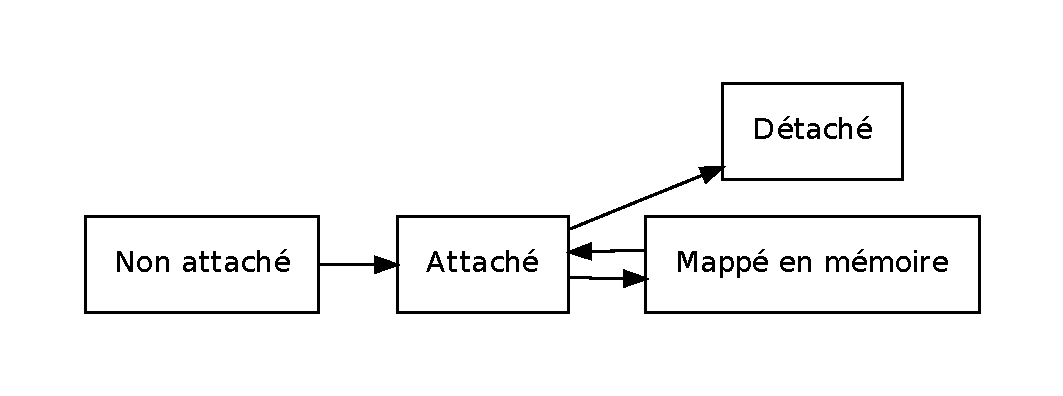
\includegraphics[width=\textwidth]{img/etatMemoirePartagee.pdf}
\end{figure}
}
{}
